\documentclass[12pt]{csethesis}
\usepackage[english]{babel}
\usepackage{amsmath}        % Extra math definitions
\usepackage{graphics}       % PostScript figures
\usepackage{setspace}       % 1.5 spacing
\usepackage{multicol}
\usepackage{bigints}
\usepackage{amssymb}
\usepackage{graphicx}
\usepackage{footnote}
\usepackage{lscape}
\usepackage{color}
\usepackage{array}
\usepackage{multirow}
\usepackage{sidecap}
\usepackage[table]{xcolor}
\usepackage{colortbl}
\usepackage{sidecap}
\usepackage{longtable}
\usepackage{wrapfig}
%\usepackage{hyperref}
\newtheorem{lemma}{Lemma}[chapter]
\makeatletter
\@addtoreset{lemma}{chapter}
\makeatother
\newtheorem{theorem}{Theorem}[chapter]
\makeatletter
\@addtoreset{theorem}{chapter}
\makeatother

\usepackage[left=1.5in,right=1in,top=1in,bottom=1in]{geometry}
%\usepackage[top=1cm,left=1cm,right=1cm,bottom=1cm]{geometry}
\usepackage{emptypage}
\usepackage{lipsum}
\usepackage{fancyhdr}
\usepackage{hyperref}
%\fancyfoot{}
%\fancyfoot{\thepage}
\fancyhead[RO,LE]{}
\fancyhead[RE]{\ifnum\value{chapter}>0 \bfseries{\nouppercase{\rightorleftmark}} \else \bfseries{\leftmark} \fi}
\fancyhead[LO]{\ifnum\value{chapter}>0 \bfseries{\nouppercase{\rightorleftmark}}  \else \bfseries{\leftmark} \fi}
%\fancyhead[LO]{ \bfseries\slshape\nouppercase{\rightorleftmark}}
\makeatletter
\newcommand{\rightorleftmark}{%
  \begingroup\protected@edef\x{\rightmark}%
  \ifx\x\@empty
    \endgroup\slshape\nouppercase{\leftmark}
  \else
    \endgroup\rightmark
  \fi}
\makeatother

\newtheorem{example}{Example}
\phdtitle = {[Title of the project]}
\name = {[Name of the student]}
\rollno = {[Roll Number]}
\guide = {[Name of Supervisor]}

\begin{document}
\pagenumbering{roman}
\begin{titlepage}
% \textheight 15.5in \textwidth 12.5in {\raggedright \huge\bf \the\phdtitle}\\[70ex]
% \begin{flushright}
% \hspace{8cm}{\LARGE \bf \the\name}\\  [1ex] 
% \end{flushright}
%\pagebreak
\thispagestyle{empty}
\mbox{}
%\pagebreak
\begin{center}
\textbf{\Huge Software Fault Detection using Isolation Forest and Deep learning }
\textheight 15.5in \textwidth 12.5in \\[9ex]
\emph{Report submitted in fulfillment of the requirements\\
for BTech Project\\
[2ex]\large \bf Third Year B.Tech.
}\\
[2ex] \emph{by} \\[2ex]

\textbf{\large Bavanya }{(18075034)}\\[1ex]
\textbf {\large Swati S Malik}{(18075060)}\\ [5ex] 
   %          \the\rollno\\[6ex]
\emph{Under the guidance of}\\[1ex]
\textbf{\large Dr.Amrita Chaturvedi} \\[7ex]


\vspace{.05in}
\begin{center}
 
\includegraphics[scale=.7,keepaspectratio=true]{./logo.jpeg}
 % iitglogo.eps: 0x0 pixel, 300dpi, 0.00x0.00 cm, bb=
\end{center}
% 

%{\sl \bf{to the}} \\[1ex]
\vspace{1cm}
{\small  \bf Department of Computer Science and Engineering}  \\[1ex]
{\small \bf{INDIAN INSTITUTE OF TECHNOLOGY (BHU) VARANASI \\
Varanasi 221005, India\\
  May 2021}}

\end{center}
\end{titlepage}

\newpage
\thispagestyle{empty}
\mbox{}
%\onehalfspacing
\doublespacing
\chapter*{ }
\label{dedication}
\thispagestyle{empty}
\begin{center}
% \large\bf \lq\lq{}Om Vang Me Manasi Pratisthita\rq\rq{}\\
% \sl \lq\lq{}May my mind be stable in my speech, May Atman manifest  \\
% \sl unto me and reveal unto me the Highest Knowledge\rq\rq{}\\
% \bf-Aitareya Upanishad\\[18ex]
%\large\bf  In Memory of\\
%\large\bf  Dadu, Thakurda and Thakuma\\[18ex]
\Huge\bf  Dedicated to\\
\Huge \em Our parents, teachers, and the almighty god.....\\[20ex]
\end{center}


\raggedbottom
\chapter*{\centering \underline{Declaration}}
\thispagestyle{empty}
We certify that
\begin{enumerate}
\item The work contained in this report is original and has been done by ourselves and the general supervision of our supervisor.
\item The work has not been submitted for any project.
\item Whenever we have used materials (data, theoretical analysis, results) from
other sources, we have given due credit to them by citing them in the text
of the thesis and giving their details in the references.
\item Whenever we have quoted written materials from other sources, we have put
them under quotation marks and given due credit to the sources by citing
them and giving required details in the references.
\end{enumerate} \vskip 10ex


\begin{table}\centering
\begin{tabular}{p{6cm}p{12cm}}
Place: IIT (BHU) Varanasi &\textbf{Bavanya and Swati Malik}\\
Date: 1/5/2021  & B.Tech\\
&Department of Computer Science and Engineering,\\
&Indian Institute of Technology (BHU) Varanasi,\\
&Varanasi, INDIA 221005.
\end{tabular}
\end{table}

\raggedbottom
%\doublespacing
%\pagenumbering{roman}
\chapter*{\centering \underline{Certificate}}
\thispagestyle{empty}
\vskip 2ex \emph{\quad This is to certify that the work contained
in this report entitled \textbf{" Software Fault Detection"} 
being submitted by \textbf{Bavanya(18075034) and Swati S Malik(18075060)}
, carried out in the Department of
Computer Science and Engineering, Indian Institute of Technology (BHU) Varanasi, is a bona fide work of my supervision.} \vskip 15ex



\begin{table}\centering
\begin{tabular}{p{6cm}p{12cm}}
 & \textbf{Dr. Amrita Chaturvedi}\\
Place: IIT (BHU) Varanasi& Department of Computer Science and Engineering,\\
Date:1/5/2021 &Indian Institute of Technology (BHU) Varanasi,\\
&Varanasi, INDIA 221005.
\end{tabular}
\end{table}
\chapter*{\centering Acknowledgments}
\thispagestyle{empty}
\quad We would like to express our sincere gratitude to our supervisor Dr.Amrita Chaturvedi for their constant guidance and support during the whole project work.
\\ \vskip 2ex
\noindent Place: IIT (BHU) Varanasi \hskip 10ex {\textbf{Bavanya and Swati }}\\
Date:1/5/2021  				
\newpage
\chapter*{\centering Abstract}
{
Effective detection of software faults is an important activity of software development process. Software plays a vital role,it  tells a computer how to function.Without software, most computers would be useless. For example, a web browser is a software application that allows users to access the internet. . An operating system (OS) is also  a software program that serves as the interface between other applications and the hardware on a computer or mobile device.So software are very important in this modern world of computers.
So defect detection is an important activity during software development process.For a software development  project ,it is  highly desirable to reduce software defects.The main goal of building program patterns is to find software defects.We implemented deep learning models with different feature extraction techniques to detect the defects in dataset.
}

 

\pagestyle{fancy}
\tableofcontents
\clearpage
\addcontentsline{toc}{chapter}{\listfigurename}
\listoffigures
%\newpage
\thispagestyle{empty}
\mbox{}
%\clearpage


\chapter{Introduction}\label{chap1}
\section{Software}
Software is a set of instructions, data, or programs used to operate a computer and execute specific tasks.Software tells a computer how to function.Without software, most computers would be useless. For example, a web browser is a software application that allows users to access the internet. . An operating system (OS) is also  a software program that serves as the interface between other applications and the hardware on a computer or mobile device.So software are very important in this modern world of computers.

\section{Software Fault Detection }
Effective detection of software faults is an important activity of software development process. Defect detection is an important activity during software development process.For a software development  project ,it is  highly desirable to reduce software defects.The main goal of building program patterns is to find software defects.\cite{software}

The main difficulty of detecting software fault is finding faults in a large and complex software system. 

\section{Unsupervised Anomaly Detection}
Anomaly detection is the method of identifying data points in the dataset which are unexpected compared to the rest of the data points.

  In case the dataset available for software fault prediction of a project is unlabelled, the fault detection problem can be handled as an Anomaly detection problem where all the faulty data points will be treated as anomalies. This approach is based on the assumption that the percentage of faulty data points is very less in the entire dataset that they can be considered as anomalies.
  
\section{Cross Version Fault Prediction}
  Metrics are extracted from a software project's specific version's source code and immediate next version's source code. Now specific version's data collected are collectively taken as the training data for training the model and the immediate next version's data collected as the collective testing data.

\section{Project Overview}
Initially we have explored Software fault detection of an unlabelled dataset as an Anomaly detection problem and later we have build different deep learning architectures for predicting faulty data points in the software fault prediction dataset.

\subsection{Different Techniques Used: }
\begin{itemize}
  \item Isolation Forest
  \item Artificial Neural Network
  \item Convolution Neural Network
  \item Recurrent Neural Network
  \item Long Short Term Memory 
  \item Gated Recurrent Unit
\end{itemize}

\subsection{Goal of Software Fault Prediction}
\begin{itemize}
  \item The main goal of software fault prediction is to use the underlying properties of the source code of a software project to predict faults before the actual testing process begins. This will help in prioritizing the work in the testing process.
\end{itemize}

\section{Organisation of the Report}\label{sec1.3}
The chapter 2 of the report explains the dataset features and the work done. Chapter 3 discusses the preprocessing, oversampling, postprocessing methods and  evaluation metrics used in detail with their working explained. In chapter 4, we give clear explanation of the models and architectures experimented for the project. In chapter 5, we display the results and the plots of the training curves to visualize the performance of the models for software fault prediction and analyse and compare the results. In chapter 6, we finally conclude and discuss the future directions of this project.

\chapter{Dataset and work done}\label{final}
\section{Dataset}\label{sec2.1}
 The datasets for training and testing the models are taken from the PROMISE repository which consists of 41 different versions of projects. The datasets are taken from 11 open source projects. Data is collected from three or more versions from each of the open source projects.
 
 We used former version of a project as the training data of our models and tested the models' predictions on the latter version for the deep learning regression models developed.
 For anomaly detection, we have taken csv files of all versions and concatenated them to a single dataset, removed the labels and split the training and testing data to 4:1 ratio for the isolation forest model.
 
 The target variable of datasets taken for anomaly prediction had binary values i.e 0 or 1 where 1 meant that a specific data point was flawed and 0 meant that it was unflawed. Whereas, for the deep learning regression problem we took that the datasets which had the target value as the number of faults corresponding to each data point.

\section{Description of Dataset}\label{sec2.2}
The following matrics are proposed by Chidamber and Kemerer, Henderson-Sellers, Martins, QMOOD and Tang et al.
The features in the datasets taken are: 

%Please add the following packages if necessary:
%\usepackage{booktabs, multirow} % for borders and merged ranges
%\usepackage{soul}% for underlines
%\usepackage[table]{xcolor} % for cell colors
%\usepackage{changepage,threeparttable} % for wide tables
%If the table is too wide, replace \begin{table}[!htp]...\end{table} with
%\begin{adjustwidth}{-2.5 cm}{-2.5 cm}\centering\begin{threeparttable}[!htb]...\end{threeparttable}\end{adjustwidth}
\begin{table}[!htp]\centering
\caption{Dataset Features}\label{tab: }
\scriptsize
\begin{tabular}{lrr}\toprule
Abbreviation &Dataset Features \\
CBO &Coupling between objects \\\midrule
RFC &Response for a class \\
LCOM &Lack of cohesion in methods \\
NOC &Number of children \\
DIT &Depth of inheritance \\
WMC &Weighted methods per class \\
Ca &Afferent couplings \\
Ce &Efferent Couplings \\
NPM &Number of public methods \\
DAM &Data Access Metric \\
MOA &Measure of Aggregation \\
MFA &Measure of Functional Abstraction \\
CAM &Cohesion Among Methods of Class \\
AMC &Average Method Complexity \\
LOC &Line of Code \\
CBM &Coupling Between Methods \\
IC &Inheritance Coupling \\
\bottomrule
\end{tabular}
\end{table}

%Please add the following packages if necessary:
%\usepackage{booktabs, multirow} % for borders and merged ranges
%\usepackage{soul}% for underlines
%\usepackage[table]{xcolor} % for cell colors
%\usepackage{changepage,threeparttable} % for wide tables
%If the table is too wide, replace \begin{table}[!htp]...\end{table} with
%\begin{adjustwidth}{-2.5 cm}{-2.5 cm}\centering\begin{threeparttable}[!htb]...\end{threeparttable}\end{adjustwidth}
\begin{table}[!htp]\centering
\caption{Explanation of the features}\label{tab: }
\scriptsize
\begin{tabular}{lrr}\toprule
Abbreviation &Explanation \\
CBO &counts the number of other classes to which a class is coupled with. \\\midrule
RFC &counts the number of external and internal classes. \\
LCOM &measures dissimilarity of methods in a class. \\
NOC &counts the number of descendants of a class. \\
DIT &measures number of ancestor classes. \\
WMC &counts the number of methods in a class weighted by complexity. \\
Ca &counts how many other classes use a given class. \\
Ce &counts the number of classes. a class is dependent upon. \\
NPM &counts the number of public methods in a class. \\
DAM &the number of private methods divided by the total number of methods. \\
MOA &counts the number of abstract data types in a class. \\
MFA &the number of inherited methods divided by total number of methods accessible by its member functions. \\
CAM &based upon the parameters in a method. \\
AMC &counts average size of method in a class. \\
LOC &counts the number of lines of source code. \\
CBM &counts the newly added func- tions with which inherited based methods are coupled. \\
IC &it is based upon inheritance-based coupling. \\
\bottomrule
\end{tabular}
\end{table}

\section{Work done}\label{sec2.3}

This section gives the overview of the work done and includes all the concepts and work done in the experiments. Indetailed explanation about each concept and term used the following subsections will be given the following next two chapters. 

\subsection{Anomaly Detection}
Data files of all the versions of a project are concatenated into a single dataframe and features without unique values are trimmed. The data did not include any null values to handle and the percentage of faulty datapoints was found to be 4.7090517241379315 \%. Applying normalization will result in the outliers not being too distinctive from the rest of the data points, so feature scaling was not applied on the dataset. Scatter plots and distribution plots were obtained of the dataset for each feature and analysed. From the plots, the distinctive behaviour of the defective data points was clearly perceivable. The data set was visualized in 3D and 2D space using t-SNE. We noticed that the data points were not distinctive in 2D or 3D space. So, we went with the earlier finalized features and didn't opt for further feature selection. We removed the labels from our data to treat the problem as unsupervised and split the training and testing data to 4:1 ratio. We used IsolationForest() function from sklearn package for building the model. To evaluate the performance of the model built, we calculated the metrics in confusion matrix and calculated the model accuracy which came out to be 87.70576131687243 \%. 

The detailed flow chart 
of the entire experiment is
given:

 \begin{figure}
\makebox[\textwidth][c]{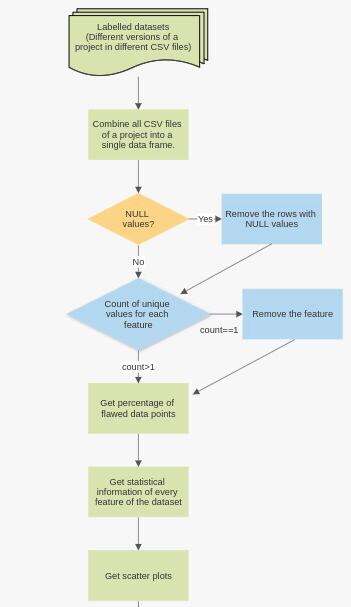
\includegraphics[width=0.6\textwidth]{others/flow1.jpeg}}%
  \caption{Flowchart of the anomaly detection experiment}
  \label{fig:key}
\end{figure}

 \begin{figure}
\makebox[\textwidth][c]{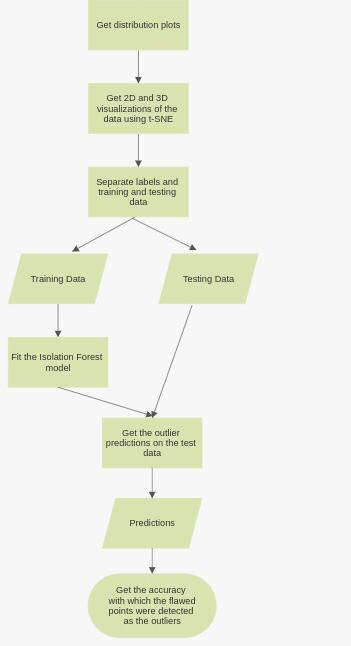
\includegraphics[width=0.6\textwidth]{others/flow2.jpeg}}%
  \caption{Flowchart continuation}
  \label{fig:key}
\end{figure}

\subsection{Regression using Deep Learning}

Exploratory data analysis has been done on the two versions of the project which were taken for training and testing the model. The analysis included checking the presence of null data points, making sure all the features had unique values for the datasets, checking the datatypes of the features and visualizing the scatter plot and frequency distribution of the data for each feature. As per the analysis done, no data cleaning or feature filteration was needed. A specific version ant-1.3 was taken to train the data and ant-1.4 version was taken for testing the models built. Min Max scaling was applied and models' performance were checked with and without different two feature reduction techiniques: SVD and PCA with each taking two different number of components hyperparameter values. Since the data points in the training and testing datasets were very few and might be inadequate for the deep learning models to learn efficiently, we used RandomOverSampler() and SMOTE() functions from imblearn package to increase the size of the data and balance it. The models were developed using tensorflow keras in python. We obtained the training and testing time of the models using the time() function from time package. The predictions obtained were round off to the nearest integer using np.rint() from numpy package because the target value to be predicted was a strict integer. Following the decision in the paper Ridge and Lasso Regression Models for Cross-Version Defect Prediction by Xiaoxing Yang and Wushao Wen we have considered FPA(Fault-percentile-average) and CLC(Cumulative lift chart (also the area under CLC)) as our main model evaluation metrics. At the end of each experiment we have automated the saving of the model weights and results in csv. 

The detailed flow chart of the experiments done for regression using deep learning is given:

 \begin{figure}
\makebox[\textwidth][c]{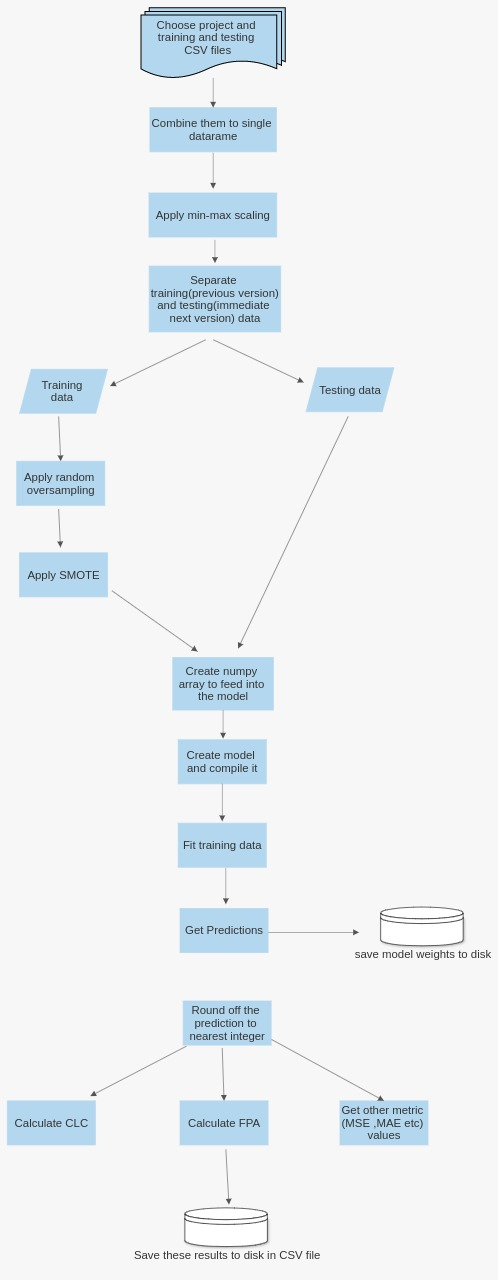
\includegraphics[width=0.6\textwidth]{others/flow_reg.jpeg}}%
  \caption{Flowchart of the anomaly detection experiment}
  \label{fig:key}
\end{figure}
\chapter{Feature Engineering and metrics}\label{final}

The feature engineering concepts used in the experiments i.e preprocessing, postprocessing and oversampling and the metrics considered for the model evaluation are discussed here.Each section is related to each of the two experiments conducted.
Each concept used in the respective type of experiment is explained in each sub section of the sections.

\section{Anomaly detection}
Extensive exploratory data analysis and preprocessing was performed on the datasets before developing the Isolation forest model. The concepts used for anomaly detection were:

\subsection{t-SNE(t-distributed stochastic neighbor embedding)}
t-SNE is used to visualize high dimensional data. The similarities between the data points are converted to joint probabilities and the Kullback-Leibler divergence between these joint probabilities of the low-dimensional embedding and the high-dimensional data is minimized. The similarities between the pairs of instances in the high dimensional space and low dimensional space are optimized using a cost function.

\section{Deep leaning regression}
Deep learning models are built to predict the number of faults corresponding to a datapoint in the testing dataset. Since the predictions are strictly greater than zero we have used ReLU Activation function after the output layer in the models and post processing is performed after that to convert the predictions to whole numbers. Different concepts used in the feature engineering in these experiments are:

\subsection{Min Max Scaling}
Min Max scaling is done to rescale a feature or observation value to a distribution value between 0 and 1. The formula followed is:
 \begin{figure}
\makebox[\textwidth][c]{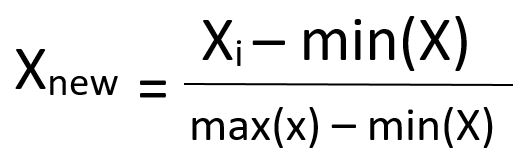
\includegraphics[width=0.2\textwidth]{others/minmaxscaling.jpg}}%
  \caption{Min Max scaling formula}
  \label{fig:key}
\end{figure}

\subsection{SVD(Singular Value Decomposition)}
The singular value decomposition (SVD) is a factorization of a real or complex matrix that generalizes the eigendecomposition of a square normal matrix to any. matrix via an extension of the polar decomposition.

\subsection{PCA(Principal Component Analysis)}
Principal Component Analysis, or PCA, is a dimensionality-reduction method that is often used to reduce the dimensionality of large data sets, by transforming a large set of variables into a smaller one that still contains most of the information in the large set.
Reducing the number of variables of a data set naturally comes at the expense of accuracy, but the trick in dimensionality reduction is to trade a little accuracy for simplicity. 


\subsection{Over Sampling}
Oversampling  in data analysis are techniques used to adjust the class distribution of a data set.
The bias in the training dataset can influence many machine learning algorithms, leading some to ignore the minority class entirely.To address this problem ,oversampling is carried out on the dataset .Random Oversampling involves supplementing the training data with multiple copies of some of the minority classes. Oversampling can be done more than once.
\subsubsection{Synthetic Minority Over-sampling Technique(SMOT)}
The most common technique to oversample a dataset used in a typical classification problem is SMOTE: Synthetic Minority Over-sampling Technique.To illustrate how this technique works consider some training data which has s samples, and f features in the feature space of the data. Note that these features, for simplicity, are continuous. As an example, consider a dataset of birds for classification. The feature space for the minority class for which we want to oversample could be beak length, wingspan, and weight (all continuous). To then oversample, take a sample from the dataset, and consider its k nearest neighbors (in feature space). To create a synthetic data point, take the vector between one of those k neighbors, and the current data point. Multiply this vector by a random number x which lies between 0, and 1. Add this to the current data point to create the new, synthetic data point.\cite{smot}

\subsection{FPA(Fault-percentile-average)}
Considering m modules f1 , f2 , . . . ,fm listed in increasing order of predicted defect number, si as the actual defect number in the module fi, and s = s1 + s2 + ... + sm as the total number
of defects in all the modules, the proportion of actual defects in the top t predicted modules (i.e., top t modules predicted to have most defects) to the whole defects is \(\frac{1}{s}\sum_{i=m-t+1}^{m}s_i\). Then FPA is defined as follows:
\[\frac{1}{m}\sum_{t=1}^{m} \frac{1}{s}\sum_{i=m-t+1}^{m}s_i\] 

\subsection{CLC(Cumulative lift chart (also the area under CLC))}

\cite{clc}CLC uses percentages of modules as x-axis and percentages of defects as y-axis. The area under CLC is always used for comparison, and the area is simply denoted as CLC in this paper.Considering m modules f1 , f2 , ..., fm , listed in increasing order of predicted defect number, si as the actual defect number in the module fi, and s = s1 + s2 + ... + sm as the total number of defects in all the modules, the area under the curve should be computed as the sum of areas of trapezoid composed of two adjacent points and the axes in the CLC. Using CLC to denote
the area under the curve in rest of the paper, it can be computed as follows:
\[CLC = \sum_{t=1}^{m}trapezoid_t\]
\[=(\frac{1}{m})(\frac{1}{2})((0+\frac{s_m}{s}+...\]
\[+(\frac{s_m+...+s_2}{s}+\frac{s_m+....+s_1}{s}))\]


\chapter{Models}\label{final}

\section{Artificial Neural Network(ANN)}
Artificial Neural Networks are a special type of machine learning algorithms that are modeled after the human brain. That is, just like how the neurons in our nervous system are able to learn from the past data, similarly, the ANN is able to learn from the data and provide responses in the form of predictions or classifications.ANNs are nonlinear statistical models which display a complex relationship between the inputs and outputs to discover a new pattern.\cite{models}
 In a neural network, there are three essential layers –
 \begin{itemize}
     \item  Input Layer- It is the first layer of an ANN that receives the input information in the form of various texts, numbers, audio files, image pixels, etc.
     \item Hidden Layer - In the middle of the ANN model are the hidden layers. There can be a single hidden layer, as in the case of a perceptron or multiple hidden layers. These hidden layers perform various types of mathematical computation on the input data and recognize the patterns that are part of.
     \item Outer Layer -In the output layer, we obtain the result that we obtain through rigorous computations performed by the middle layer.
 \end{itemize}
 
 \begin{figure}
\makebox[\textwidth][c]{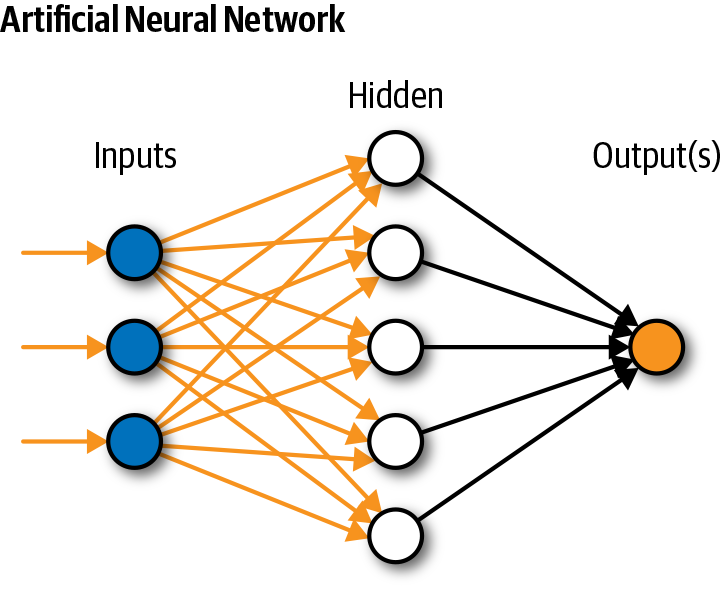
\includegraphics[width=0.6\textwidth]{others/ann.png}}%
  \caption{ANN}
  \label{fig:key}
\end{figure}
\section{Recurrent neural network(RNN)}
A recurrent neural network is a class of artificial neural networks where connections between nodes form a directed graph along a temporal sequence. This allows it to exhibit temporal dynamic behavior.It is derived from feedforward neural networks, RNNs can use their internal state (memory) to process variable length sequences of inputs.The term “recurrent neural network” is used indiscriminately to refer to two broad classes of networks with a similar general structure, where one is finite impulse and the other is infinite impulse. Both classes of networks exhibit temporal dynamic behavior.Both finite impulse and infinite impulse recurrent networks can have additional stored states, and the storage can be under direct control by the neural network. The storage can also be replaced by another network or graph, if that incorporates time delays or has feedback loops.\cite{rnn}
\begin{figure}
\makebox[\textwidth][c]{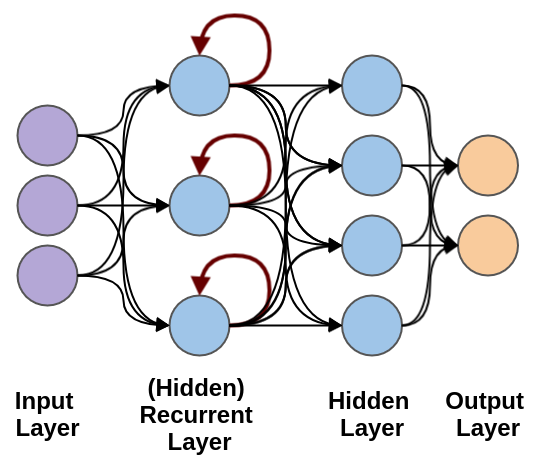
\includegraphics[width=0.6\textwidth]{others/rnn-multihidden.png}}%
  \caption{Recurrent neural network}
  \label{fig:key}
\end{figure}
\section{Long short-term memory (LSTM) }
Long Short-Term Memory (LSTM) networks are a type of recurrent neural network capable of learning order dependence in sequence prediction problems.LSTMs have the  ability to preserve long-term memory and  have a slightly more complex structure. At each time step, the LSTM cell takes in 3 different pieces of information -- the current input data, the short-term memory from the previous cell (similar to hidden states in RNNs) and lastly the long-term memory.The short-term memory is commonly referred to as the hidden state, and the long-term memory is usually known as the cell state.The cell then uses gates to regulate the information to be kept or discarded at each time step before passing on the long-term and short-term information to the next cell.These gates are called the Input Gate, the Forget Gate, and the Output Gate.\cite{lstm}
\begin{figure}
\makebox[\textwidth][c]{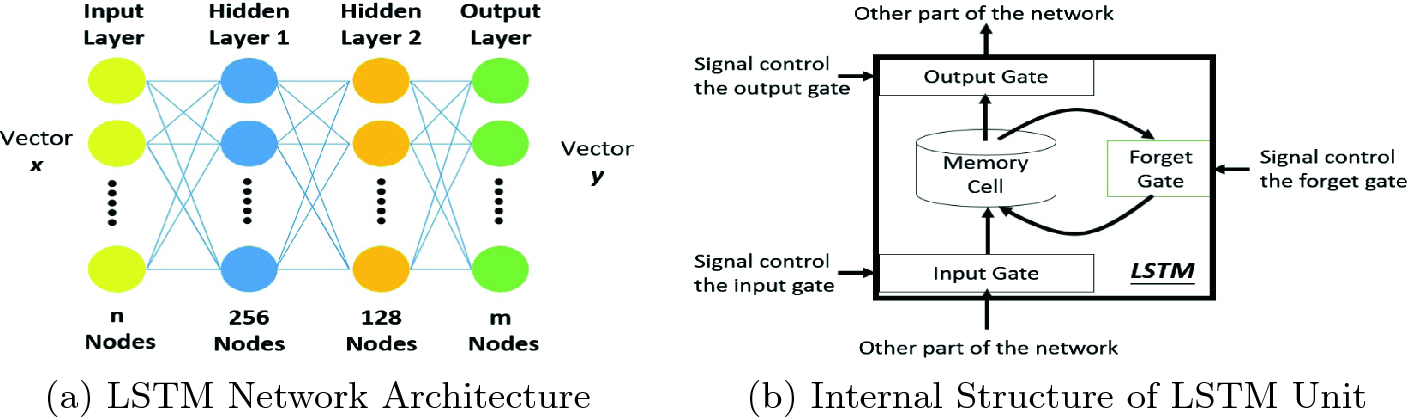
\includegraphics[width=1.2\textwidth]{others/lstm.png}}%
  \caption{LSTM}
  \label{fig:key}
\end{figure}
\section{ Gated Recurrent Unit(GRU)}
A Gated Recurrent Unit is a variant of the RNN architecture, and uses gating mechanisms to control and manage the flow of information between cells in the neural network.The structure of the GRU allows it to adaptively capture dependencies from large sequences of data without discarding information from earlier parts of the sequence. This is achieved through its gating units, similar to the ones in LSTMs, which solve the vanishing gradient problem of traditional RNNs. These gates are responsible for regulating the information to be kept or discarded at each time step.The GRU cell contains only two gates: the Update gate and the Reset gate.These gates in the GRU are trained to selectively filter out any irrelevant information while keeping what’s useful. These gates are essentially vectors containing values between 0 to 1 which will be multiplied with the input data and/or hidden state.
A 0 value in the gate vectors indicates that the corresponding data in the input or hidden state is unimportant and will, therefore, return as a zero. On the other hand, a 1 value in the gate vector means that the corresponding data is important and will be used.
\begin{figure}
\makebox[\textwidth][c]{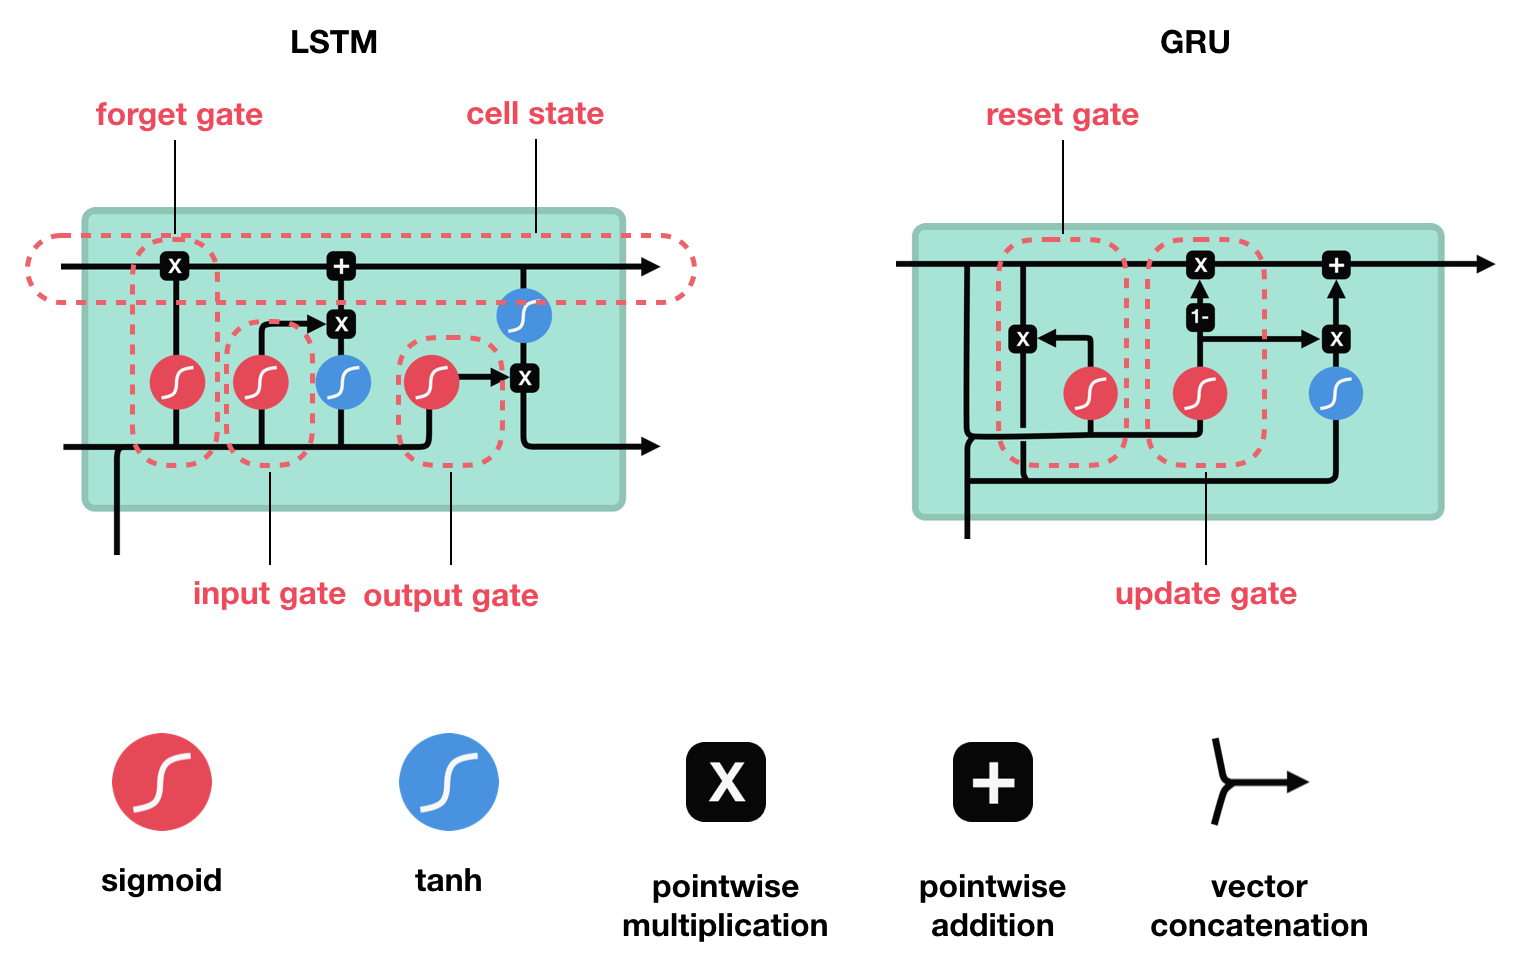
\includegraphics[width=0.8\textwidth]{others/gru.png}}%
  \caption{LSTM vs GRU}
  \label{fig:key}
\end{figure}
\section{ Convolutional Neural Network (CNN)}
In deep learning, a convolutional neural network (CNN, or ConvNet) is a class of deep neural network, most commonly applied to analyze visual imagery
We track sizes of communities across time.
As the community labels are changing, we keep track of size changes by cluster memberships.CNNs are regularized versions of multilayer perceptrons. Multilayer perceptrons usually mean fully connected networks, that is, each neuron in one layer is connected to all neurons in the next layer.A convolutional neural network consists of an input layer, hidden layers and an output layer. In any feed-forward neural network, any middle layers are called hidden because their inputs and outputs are masked by the activation function and final convolution. In a convolutional neural network, the hidden layers include layers that perform convolutions. \cite{cnn}

\begin{figure}
\makebox[\textwidth][c]{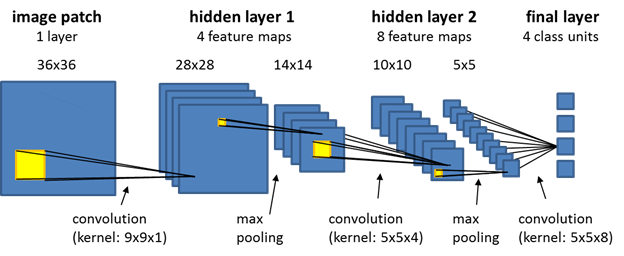
\includegraphics[width=0.8\textwidth]{others/cnn.png}}%
  \caption{CNN}
  \label{fig:key}
\end{figure}


\section{Isolation Forest}
Isolation forest is an unsupervised learning algorithm for anomaly detection that works on the principle of isolating anomalies,instead of the most common techniques of profiling normal points.An anomaly is an observation or event that deviates so much from other events to arouse suspicion it was generated by a different mean.Anomalies in a big dataset may follow very complicated patterns, which are difficult to detect “by eye” in the great majority of cases.In order to isolate a data point(outlier), the algorithm recursively generates partitions on the sample by randomly selecting an attribute and then randomly selecting a split value for the attribute, between the minimum and maximum values allowed for that attribute.\cite{isolationF}
\begin{figure}
\makebox[\textwidth][c]{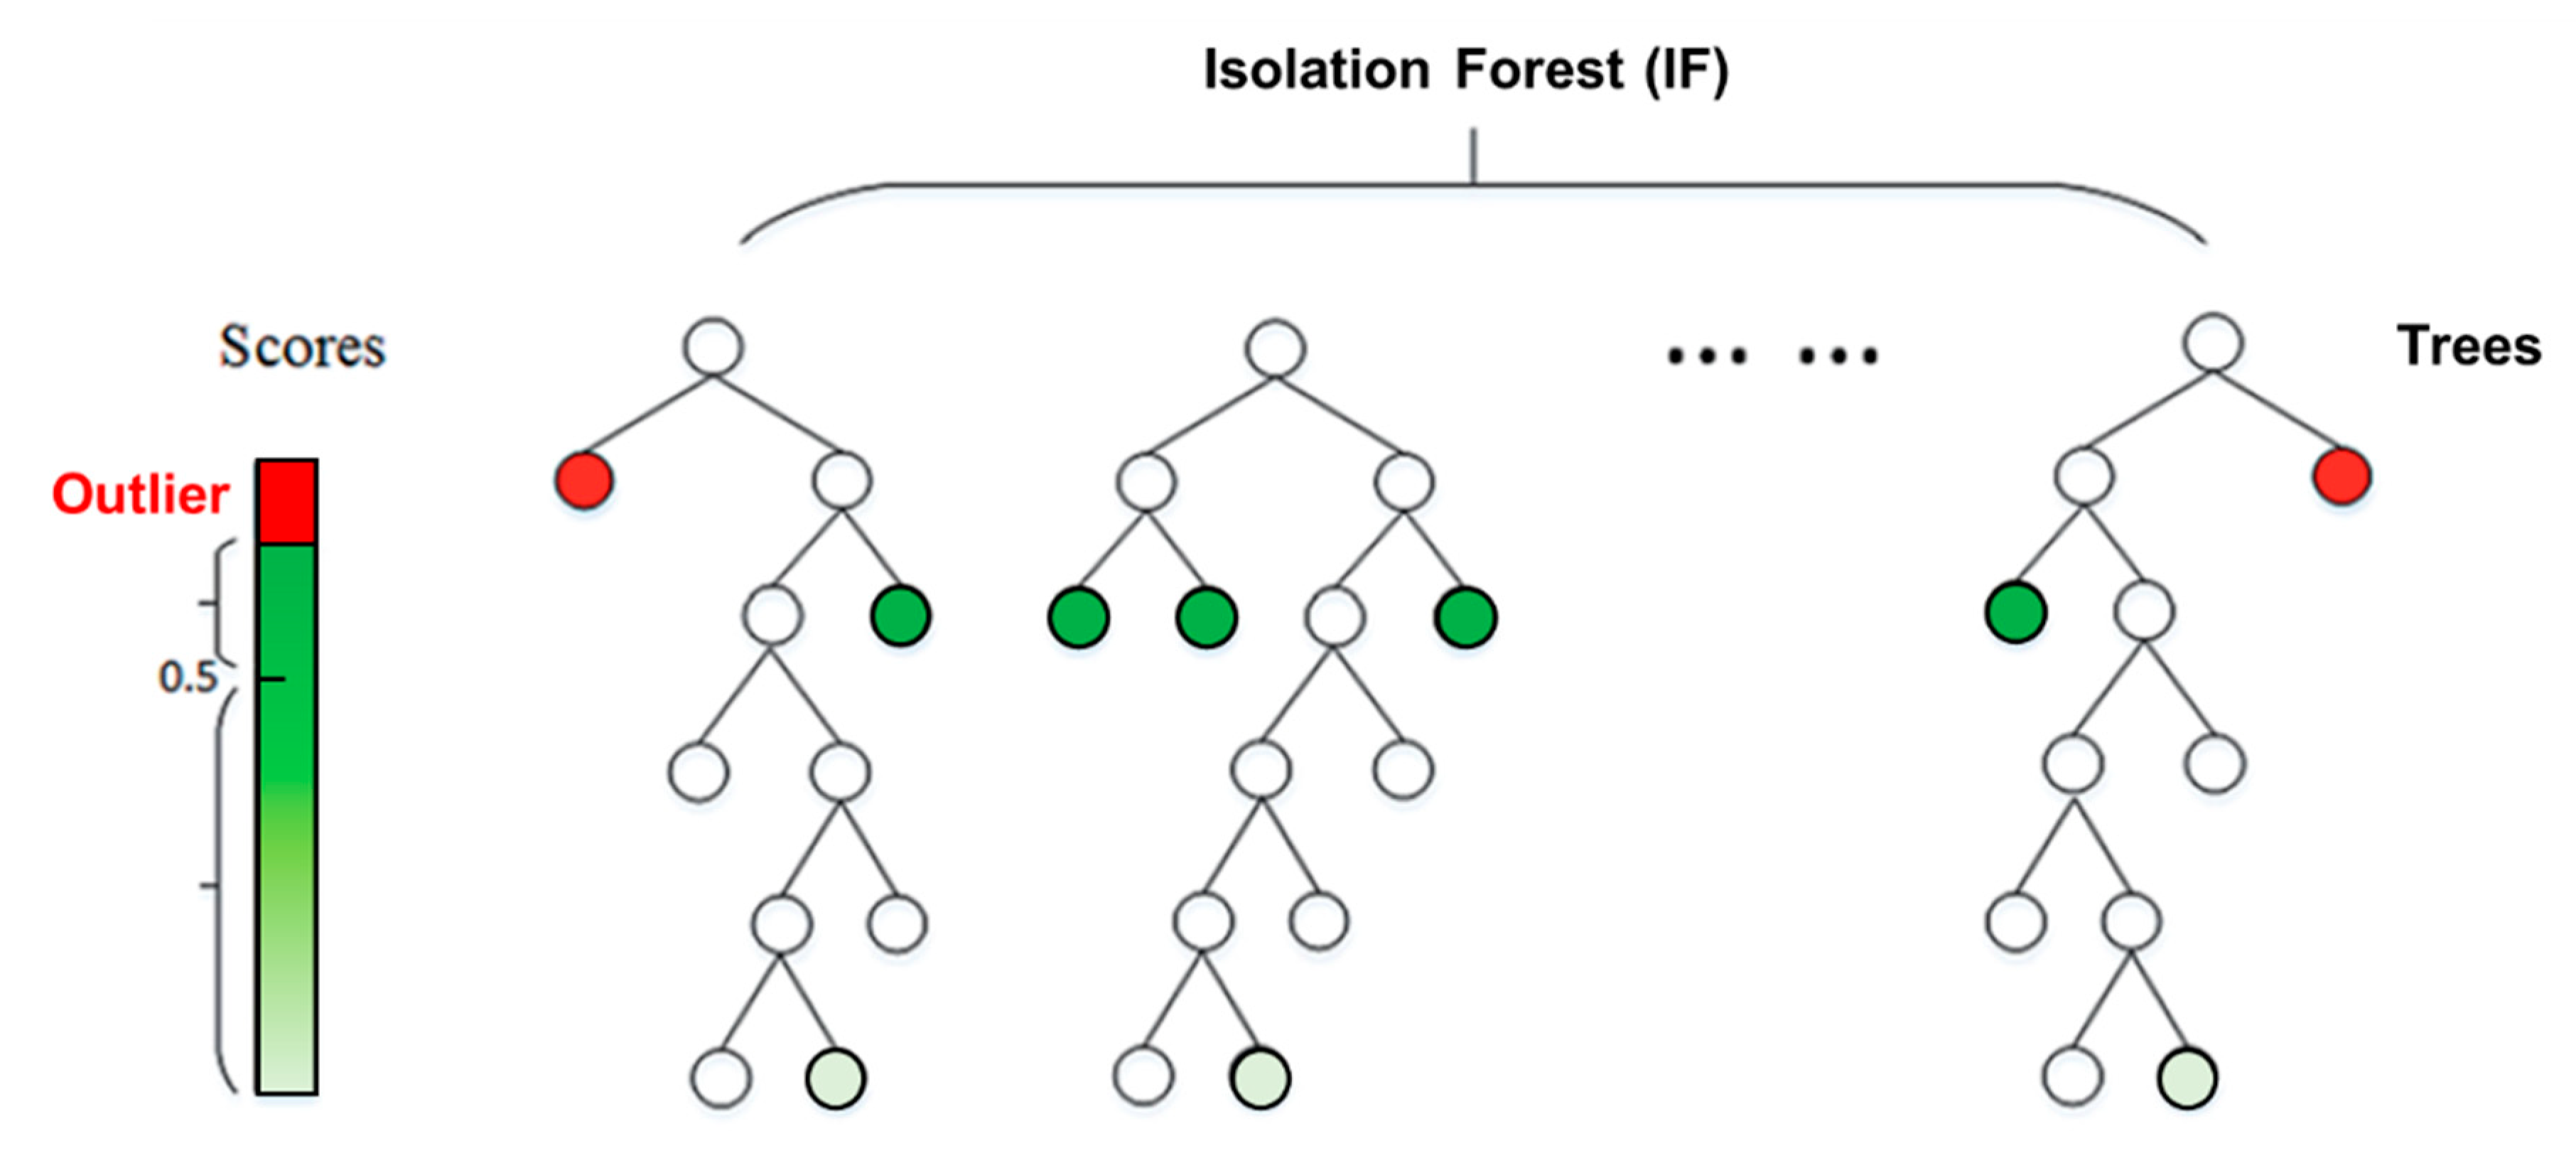
\includegraphics[width=0.8\textwidth]{others/isolation.png}}%
  \caption{Isolation Forest}
  \label{fig:key}
\end{figure}





 
\chapter{Results}\label{final}

\section{Anomaly detection}

Using Isolation Forest we have performed anomaly detection to detect the faulty datapoints in the datasets. The 2D and 3D visualizations from t-SNE are as follows:

\begin{figure}
\makebox[\textwidth][c]{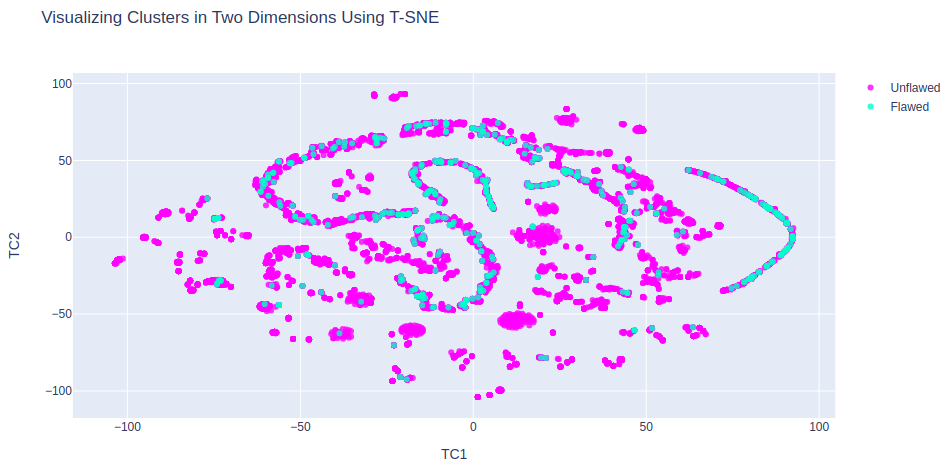
\includegraphics[width=0.8\textwidth]{others/2d_tsne.png}}%
  \caption{2D visualization}
  \label{fig:key}
\end{figure}

\begin{figure}
\makebox[\textwidth][c]{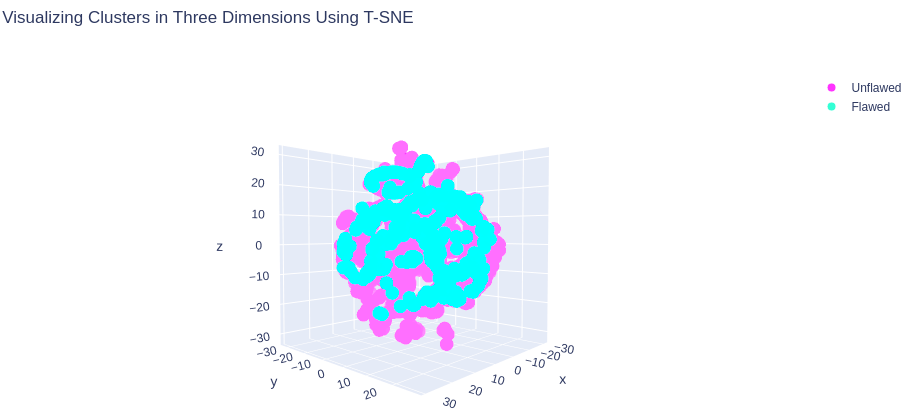
\includegraphics[width=0.8\textwidth]{others/3d_tsne.png}}%
  \caption{3D visualization}
  \label{fig:key}
\end{figure}

From the visualizations, it became clear that extensive feature reduction would not help in detecting the faulty datapoints. So, we proceeded without any feature selection. 
The datasets taken were initially labelled, so we found out the percentage of the faulty datapoints which came out to be 4.71 \% and plotted the distribution of the labels before removing the labels. The plot obtained is: 

\begin{figure}
\makebox[\textwidth][c]{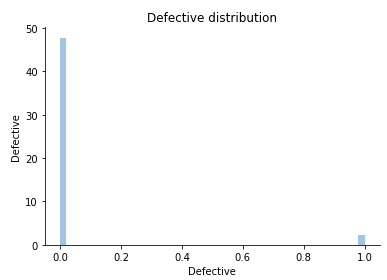
\includegraphics[width=0.8\textwidth]{others/defect_distribution.png}}%
  \caption{Distribution of labels}
  \label{fig:key}
\end{figure}

After applying the Isolation Forest model, we have obtained the Accuracy of the model by obtaining true positive, true negative and all samples count in the predictions. The formula for accuracy used is:

\[\frac{True Positive + True Negative}{All Samples}\] 

\section{Deep Learning Regression}
We performed 32 experiments without any feature selection and with three different feature selection techniques:
 \begin{itemize}
     \item Singular value Decomposition with 10 and 15 components
     \item Principal component analysis with 10 and 15 components
     \item Information Gain
 \end{itemize}
and each of SVD and PCA with two different number of components: 10 and 15.
Min Max scaling preprocessing was performed on the datasets before running all the models. The predictions obtained by all the models were rounded off to nearest integers. We used MSE as the loss function for all the models
We have developed 9 different models and tried 3 different architectures of LSTM, 3 different architectures of RNN and single architecture each of GRU, ANN and CNN.

\subsection{ANN}
The schematics of the ANN model designed is visualized as follows:

\begin{figure}
\makebox[\textwidth][c]{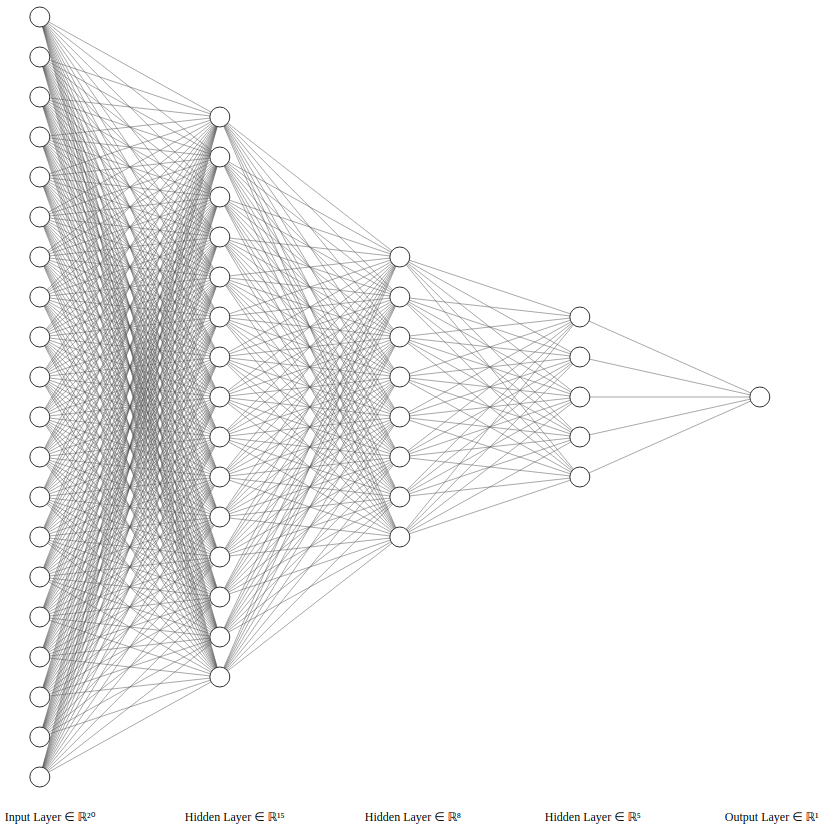
\includegraphics[width=0.8\textwidth]{others/nn.png}}%
  \caption{ANN Architecture}
  \label{fig:key}
\end{figure}
 
 The performance results are as follows:
 
%Please add the following packages if necessary:
%\usepackage{booktabs, multirow} % for borders and merged ranges
%\usepackage{soul}% for underlines
%\usepackage[table]{xcolor} % for cell colors
%\usepackage{changepage,threeparttable} % for wide tables
%If the table is too wide, replace \begin{table}[!htp]...\end{table} with
%\begin{adjustwidth}{-2.5 cm}{-2.5 cm}\centering\begin{threeparttable}[!htb]...\end{threeparttable}\end{adjustwidth}
\begin{table}[!htp]\centering
\caption{ANN Model results}\label{tab: }
\scriptsize
\begin{tabular}{lrrrrrr}\toprule
Feature Selection &No. of components &FPA &CLC &Train Loss at last epoch(MSE) &Test Loss(MSE) \\
\textbf{N/A} &\textbf{N/A} &\textbf{0.47545615} &\textbf{0.48384327} &\textbf{0.555} &\textbf{1.1668} \\\midrule
SVD &10 &0.47456595 &0.48294193 &0.385 &0.907 \\
SVD &15 &NAN &NAN &3.5 &0.3652 \\
PCA &10 &NAN &NAN &3.5 &0.3652 \\
PCA &15 &0.4627341 &0.47109878 &0.2115 &0.8144 \\
\bottomrule
\end{tabular}
\end{table}
 
Observing the results, we can see that the FPA and CLC is obtained to be NAN for two of the experiments. This situation is encountered when all the predictions i.e the number of bugs in the testing data come out to be zero after rounding off. This is an unwanted result. We also see that the best FPA and CLC are obtained when no feature selection technique is applied.

\subsection{GRU}
The schematics of the GRU model designed is visualized as follows:

\begin{figure}
\makebox[\textwidth][c]{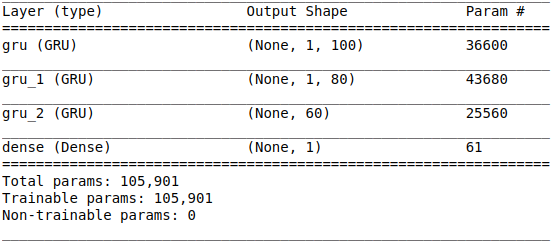
\includegraphics[width=0.8\textwidth]{others/gru_summary.png}}%
  \caption{GRU Architecture}
  \label{fig:key}
\end{figure}

Oversampling and SMOTE were applied to all the experiments involving the GRU model also. The performance results are as follows:
 
%Please add the following packages if necessary:
%\usepackage{booktabs, multirow} % for borders and merged ranges
%\usepackage{soul}% for underlines
%\usepackage[table]{xcolor} % for cell colors
%\usepackage{changepage,threeparttable} % for wide tables
%If the table is too wide, replace \begin{table}[!htp]...\end{table} with
%\begin{adjustwidth}{-2.5 cm}{-2.5 cm}\centering\begin{threeparttable}[!htb]...\end{threeparttable}\end{adjustwidth}
\begin{table}[!htp]\centering
\caption{GRU Model results}\label{tab: }
\scriptsize
\begin{tabular}{lrrrrrr}\toprule
Feature Selection &No. of components &FPA &CLC &Train Loss at last epoch(MSE) &Test Loss(MSE) \\
N/A &N/A &0.48528624 &0.49368343 &0.9214 &1.3261 \\\midrule
SVD &10 &0.48289812 &0.49128413 &0.7384 &1.0185 \\
SVD &15 &0.47688892 &0.4852823 &0.6949 &1.2748 \\
\textbf{PCA} &\textbf{10} &\textbf{0.49431464} &\textbf{0.5027083} &\textbf{0.7483} &\textbf{1.1861} \\
PCA &15 &0.4928466 &0.5012389 &0.7455 &1.1761 \\
\bottomrule
\end{tabular}
\end{table}
 
Observing the results, we see that the best FPA and CLC are obtained when PCA is applied and 10 components were taken for training the model and the least FPA and CLC are obtained when SVD is applied and 15 components were taken for training the model.

\subsection{CNN}
The schematics of the CNN model designed is visualized as follows:

\begin{figure}
\makebox[\textwidth][c]{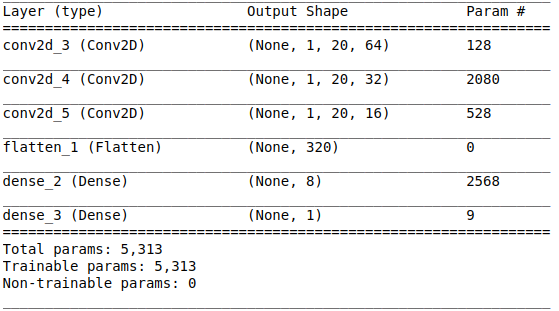
\includegraphics[width=0.8\textwidth]{others/cnn_summary.png}}%
  \caption{CNN Architecture}
  \label{fig:key}
\end{figure}

6 Experiments were conducted taking CNN model and we ran one of the experiments without applying any obersampling and smote with PCA taking 10 components. Rest of the 5 experiments were applying on oversampled and SMOTE balanced data with different feature selection techniques. The performance results are as follows:
 
%Please add the following packages if necessary:
%\usepackage{booktabs, multirow} % for borders and merged ranges
%\usepackage{soul}% for underlines
%\usepackage[table]{xcolor} % for cell colors
%\usepackage{changepage,threeparttable} % for wide tables
%If the table is too wide, replace \begin{table}[!htp]...\end{table} with
%\begin{adjustwidth}{-2.5 cm}{-2.5 cm}\centering\begin{threeparttable}[!htb]...\end{threeparttable}\end{adjustwidth}
\begin{table}[!htp]\centering
\caption{CNN Experiments Details}\label{tab: }
\scriptsize
\begin{tabular}{lrrrr}\toprule
Model Number &Feature Selection &No. of components &Oversampling and SMOTE \\
1 &N/A &N/A &yes \\\midrule
2 &SVD &10 &yes \\
3 &SVD &15 &yes \\
4 &\textbf{PCA} &\textbf{10} &\textbf{yes} \\
5 &PCA &10 &no \\
6 &PCA &15 &yes \\
\bottomrule
\end{tabular}
\end{table}

%Please add the following packages if necessary:
%\usepackage{booktabs, multirow} % for borders and merged ranges
%\usepackage{soul}% for underlines
%\usepackage[table]{xcolor} % for cell colors
%\usepackage{changepage,threeparttable} % for wide tables
%If the table is too wide, replace \begin{table}[!htp]...\end{table} with
%\begin{adjustwidth}{-2.5 cm}{-2.5 cm}\centering\begin{threeparttable}[!htb]...\end{threeparttable}\end{adjustwidth}
\begin{table}[!htp]\centering
\caption{CNN Model results}\label{tab: }
\scriptsize
\begin{tabular}{lrrrrr}\toprule
Model Number &FPA &CLC &Train Loss at last epoch(MSE) &Test Loss(MSE) \\
1 &0.484641 &0.4930281 &0.5649 &1.1203 \\\midrule
2 &0.4716726 &0.4800206 &0.094 &0.7005 \\
3 &NAN &NAN &3.5 &0.3652 \\
4 &\textbf{0.498646} &\textbf{0.507073} &\textbf{0.1769} &\textbf{0.7597} \\
5 &0.473417 &0.481844 &0.2426 &0.4125 \\
6 &0.478746 &0.487105 &0.1106 &0.743 \\
\bottomrule
\end{tabular}
\end{table}
 
Observing the results, we obtained undesired NAN values for FPA and CLC when we applied SVD and obtained 15 components. The best results were obtained when we ran the model with oversampled and SMOTE balanced data after applying PCA and obtaining 10 components. 

\subsection{LSTM}

Three different architectures were tried and they are as follows:
 \begin{itemize}
     \item Architecture 1: Three LSTM layers with decreasing output features and single dense layer at the end.
     \item Architecture 2: Five LSTM layers with decreasing output features and single dense layer at the end.
     \item Architecture 3: Seven LSTM layers with decreasing output features and single dense layer at the end.
 \end{itemize}
 
 The summaries of the three LSTM architectures tried as as follows:
 
 \begin{figure}
\makebox[\textwidth][c]{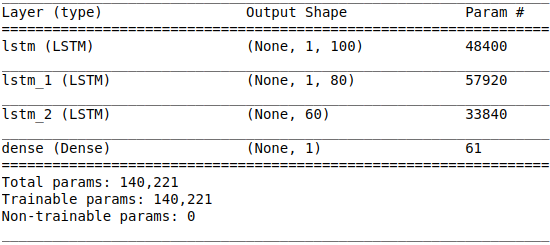
\includegraphics[width=0.8\textwidth]{others/LSTM_summary1.png}}%
  \caption{LSTM Architecture 1}
  \label{fig:key}
\end{figure}

\begin{figure}
\makebox[\textwidth][c]{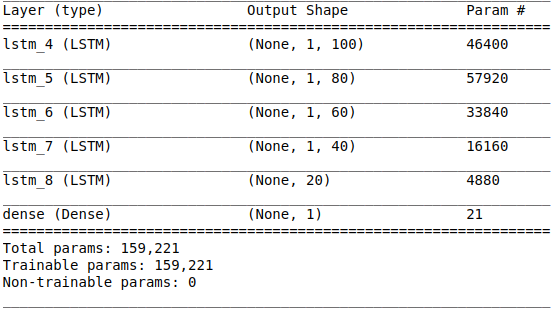
\includegraphics[width=0.8\textwidth]{others/LSTM_summary2.png}}%
  \caption{LSTM Architecture 2}
  \label{fig:key}
\end{figure}

\begin{figure}
\makebox[\textwidth][c]{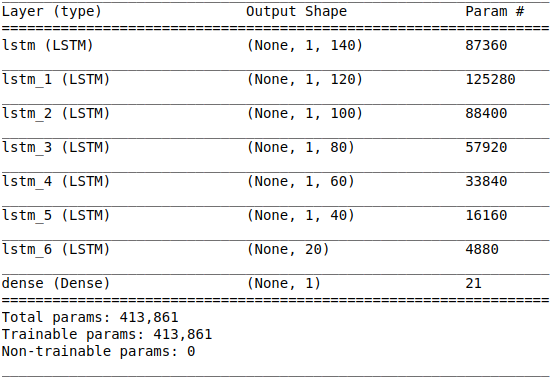
\includegraphics[width=0.8\textwidth]{others/LSTM_summary3.png}}%
  \caption{LSTM Architecture 3}
  \label{fig:key}
\end{figure}
 
Oversampling and SMOTE were applied to all the experiments involving the three LSTM models also. Info gain was taken as a feature selection criteria in one of the experiments. Considering the info gain, 9 features were selected. They are: CBO, RFC, Ce, LCOM3, LOC, DAM, MOA, MFA and CAM. The explanation of the following features are given in chapter 2.

The performance results are as follows:

%Please add the following packages if necessary:
%\usepackage{booktabs, multirow} % for borders and merged ranges
%\usepackage{soul}% for underlines
%\usepackage[table]{xcolor} % for cell colors
%\usepackage{changepage,threeparttable} % for wide tables
%If the table is too wide, replace \begin{table}[!htp]...\end{table} with
%\begin{adjustwidth}{-2.5 cm}{-2.5 cm}\centering\begin{threeparttable}[!htb]...\end{threeparttable}\end{adjustwidth}
\begin{table}[!htp]\centering
\caption{LSTM Experiments Details}\label{tab: }
\scriptsize
\begin{tabular}{lrrrr}\toprule
Model Number &Architecture Number &Feature Selection &No. of components \\
1 &1 &N/A &N/A \\\midrule
2 &1 &SVD &15 \\
3 &1 &SVD &10 \\
4 &1 &Info\_gain &9 Features selected \\
5 &1 &PCA &15 \\
6 &1 &PCA &10 \\
7 &\textbf{2} &\textbf{PCA} &\textbf{15} \\
8 &3 &PCA &15 \\
\bottomrule
\end{tabular}
\end{table}

%Please add the following packages if necessary:
%\usepackage{booktabs, multirow} % for borders and merged ranges
%\usepackage{soul}% for underlines
%\usepackage[table]{xcolor} % for cell colors
%\usepackage{changepage,threeparttable} % for wide tables
%If the table is too wide, replace \begin{table}[!htp]...\end{table} with
%\begin{adjustwidth}{-2.5 cm}{-2.5 cm}\centering\begin{threeparttable}[!htb]...\end{threeparttable}\end{adjustwidth}
\begin{table}[!htp]\centering
\caption{LSTM Model results}\label{tab: }
\scriptsize
\begin{tabular}{lrrrrr}\toprule
Model Number &FPA &CLC &Train Loss at last epoch(MSE) &Test Loss(MSE) \\
1 &0.4891348 &0.49753347 &0.9225 &1.3541 \\\midrule
2 &0.4854812 &0.4938745 &0.8029 &1.2402 \\
3 &0.48686993 &0.49526507 &0.7701 &1.2719 \\
4 &0.48584172 &0.494218 &0.9962 &1.421 \\
5 &0.49402896 &0.5024241 &0.7275 &1.2536 \\
6 &0.4832134 &0.4916067 &0.7384 &1.1761 \\
7 &\textbf{0.504664} &\textbf{0.5130555} &\textbf{0.741} &\textbf{1.2263} \\
8 &0.4919156 &0.5003081 &0.7219 &1.3139 \\
\bottomrule
\end{tabular}
\end{table}

From the table, we can observe that the best result was obtained from the LSTM model with architecture 2 when PCA was applied on the data and 15 components were obtained. The second best result was obtained from the architecture 1 of the LSTM models when PCA was obtained and 15 components were taken.

\subsection{RNN}

Three different architectures were tried and they are as follows:
 \begin{itemize}
     \item Architecture 1: Three RNN layers with decreasing output features and single dense layer at the end.
     \item Architecture 2: Five RNN layers with decreasing output features and single dense layer at the end.
     \item Architecture 3: Three RNN layers with decreasing output features and single dense layer at the end. This architecture is slightly less complex than the 1st RNN architecture.
 \end{itemize}
 
 The summaries of the three RNN architectures tried as as follows:
 
 \begin{figure}
\makebox[\textwidth][c]{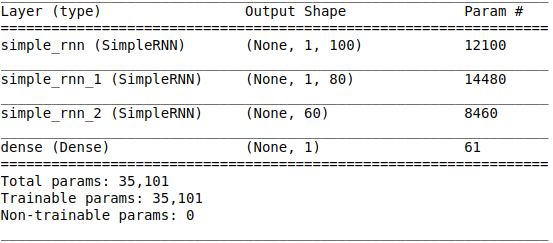
\includegraphics[width=0.8\textwidth]{others/rnn_summary1.png}}%
  \caption{RNN Architecture 1}
  \label{fig:key}
\end{figure}

\begin{figure}
\makebox[\textwidth][c]{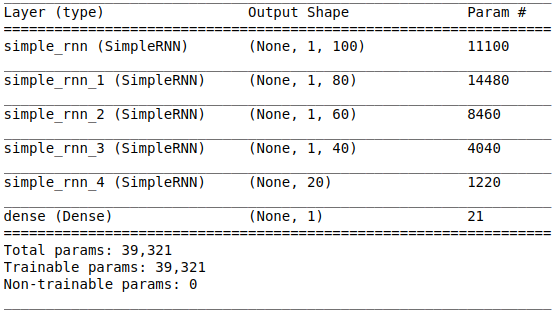
\includegraphics[width=0.8\textwidth]{others/rnn_summary2.png}}%
  \caption{RNN Architecture 2}
  \label{fig:key}
\end{figure}

\begin{figure}
\makebox[\textwidth][c]{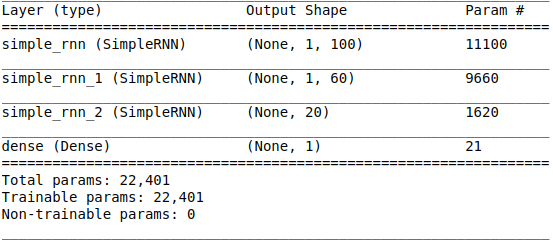
\includegraphics[width=0.8\textwidth]{others/rnn_summary3.png}}%
  \caption{RNN Architecture 3}
  \label{fig:key}
\end{figure}
 
8 experiments were performed on the RNN models of which in one experiment, we have not oversampled and SMOTE balanced the data. 

The performance results are as follows:

%Please add the following packages if necessary:
%\usepackage{booktabs, multirow} % for borders and merged ranges
%\usepackage{soul}% for underlines
%\usepackage[table]{xcolor} % for cell colors
%\usepackage{changepage,threeparttable} % for wide tables
%If the table is too wide, replace \begin{table}[!htp]...\end{table} with
%\begin{adjustwidth}{-2.5 cm}{-2.5 cm}\centering\begin{threeparttable}[!htb]...\end{threeparttable}\end{adjustwidth}
\begin{table}[!htp]\centering
\caption{RNN Experiments Details}\label{tab: }
\scriptsize
\begin{tabular}{lrrrrr}\toprule
Model Number &Architecture Number &Feature Selection &No. of components &Oversampling and SMOTE \\
1 &1 &N/A &N/A &yes \\\midrule
2 &\textbf{1} &\textbf{SVD} &\textbf{10} &\textbf{yes} \\
3 &1 &SVD &10 &no \\
4 &1 &SVD &15 &yes \\
5 &1 &PCA &10 &yes \\
6 &1 &PCA &15 &yes \\
7 &2 &SVD &10 &yes \\
8 &3 &SVD &10 &yes \\
\bottomrule
\end{tabular}
\end{table}

%Please add the following packages if necessary:
%\usepackage{booktabs, multirow} % for borders and merged ranges
%\usepackage{soul}% for underlines
%\usepackage[table]{xcolor} % for cell colors
%\usepackage{changepage,threeparttable} % for wide tables
%If the table is too wide, replace \begin{table}[!htp]...\end{table} with
%\begin{adjustwidth}{-2.5 cm}{-2.5 cm}\centering\begin{threeparttable}[!htb]...\end{threeparttable}\end{adjustwidth}
\begin{table}[!htp]\centering
\caption{RNN Model results}\label{tab: }
\scriptsize
\begin{tabular}{lrrrrr}\toprule
Model Number &FPA &CLC &Train Loss at last epoch(MSE) &Test Loss(MSE) \\
1 &0.49177 &0.50014 &0.8385 &1.3362 \\\midrule
2 &\textbf{0.50518} &\textbf{0.51357} &\textbf{0.6928} &\textbf{1.2263} \\
3 &0.49487 &0.5033 &0.3527 &0.3634 \\
4 &0.48322 &0.49161 &0.5944 &1.0027 \\
5 &0.48304 &0.49143 &0.7491 &1.1926 \\
6 &0.49248 &0.50087 &0.5342 &0.9949 \\
7 &0.49188 &0.50027 &0.644 &1.1513 \\
8 &0.47143 &0.479826 &0.6852 &1.156 \\
\bottomrule
\end{tabular}
\end{table}

From the table, we can observe that the best result was obtained when SVD was applied on oversampled and SMOTE balanced data and 10 components were selected. 

The training curve of the best performing model among the 32 experiments is plotted using tensorboard and it is visualized as follows:

 \begin{figure}
\makebox[\textwidth][c]{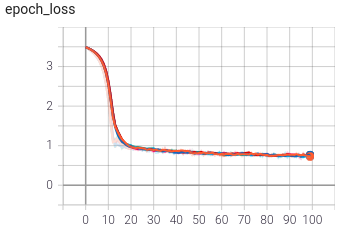
\includegraphics[width=0.8\textwidth]{others/epoch_loss.png}}%
  \caption{Training curve}
  \label{fig:key}
\end{figure}


\chapter{Conclusions and Discussion}\label{final}

\section{Conclusion}

In conclusion we see that the best performing model among all the models and different architectures is the first architecture from RNN models when SVD is applied for selecting 10 components from the dataset features after oversampling and smote balancing the data. Also a clear observation is that the ANN model performed the least compared to the other models. The remaining 4 models gave results almost close to each other. We also see that in some cases, we got NAN values for FPA and CLC but the test loss in those cases is the second least and the train loss was the highest among all the experiments. Hence taking FPA and CLC as the criteria for evalutaing the model performance was better. 

\section{Future scope}
For even more improved results, attention layers can be introduced in the model architectures. Even after taking such complex architectures the results were very close to each other and the dataset was small because of taking cross versions so we had to perform oversampling and SMOTE balancing. It is possible that due to limited data of cross versions for the training of the deep learning models, the results were saturated. Different classical Machine learning techniques could be applied on the same data and checked for better results.
\bibliographystyle{IEEEtran}
\bibliography{report}
\end{document}
